% -------------------------------------------------------------------------------------------------
%      MDSG Latex Framework
%      ============================================================================================
%      File:                  introduction-[UTF8,ISO8859-1].tex
%      Author(s):             Michael Duerr
%      Version:               1
%      Creation Date:         30. Mai 2010
%      Creation Date:         30. Mai 2010
%
%      Notes:                 - Example chapter
% -------------------------------------------------------------------------------------------------
%
\chapter{Results}\label{sec:Results}
% - Result presentation
% - Description of images and charts \\
% - One Agent Environment vs MARL
% - Best cases of reward, trades, grid coloration, field resets
% - Worst cases of above
% - influence of markets
In this chapter the results of various training executions with different parameters are compared. All possible combinations of markets, agent compositions and learning algorithms in an easy environment setup are shown in section \ref{easy_env}. The best combinations are then extracted and applied in more challenging environments, which are compared in section \ref{difficult_env}. Furthermore, Appendix \ref{ax:plots} shows all generated training plots of the presented results.

\section{Setup} \label{setup}

\marginpar{was wurde untersucht}
The results of this research compare multiagent trainings with varying settings, namely acting in different compositions and markets. In this case the amount of agents stays fixed and is greater than one. The agents use either of the two learning approaches PPO or DQN to train. Hence, the overall possible comparisons include a total amount of 102 executions. This number results from the calculation of multiplying the 2 learning algorithms with the 3 possible agent compositions (cooperative, competitive and mixed-motive) and additionally 2 optional markets that can contain 3 modular additions. 

The market options are for example the following SM instances: 
\begin{itemize}
    \item ``sm''
    \item ``sm-goal''
    \item ``sm-no-debt''
    \item ``sm-no-reset''
    \item ``sm-no-reset-no-debt''
    \item ``sm-goal-no-debt''
    \item ``sm-goal-no-reset''
    \item ``sm-goal-no-reset-no-debt''
\end{itemize}
The 8 options above are also applied on the AM and lastly the option of no market needs to be considered, leading to 17 market scenarios. Calculating the total amount of executions now with those 17 market possibilities results in the 102 executions.

\marginpar{was wurde nicht untersucht}
Yet, not all market arrangements are needed. For example, the mix of ``no-reset'' and ``no-debt'' is not of use in this implementation. An agent that has reset a field has a reward of -0.1 and therefore already is in debt, which means that ``no-debt'' includes ``no-reset''. This subtracts 4 compositions from the 17 market scenarios. Additionally, shares are free of charge, making the options ``sm-no-debt'' and ``sm-goal-no-debt'' irrelevant. Agents can always afford to buy shares in this case. The SM is therefore left with 4 combinations and the overall market scenario count is now 11. In total the analyzation only includes 66 training results. 

\marginpar{wie wurde untersucht / zahlen}
In order to compare the market approach with a credit assignment solution in the cooperation composition, the training with a DR setting is also included. This in turn adds another execution to each learning algorithm. Furthermore, to ensure that the environment is generally solvable, one agent first trains in the environment setup with each learning algorithm using similar hyperparameter as in the multiagent case. To summarize the execution count is therefore 70 in total.

Those 70 executions are mostly run with the default parameters that can be looked up in Appendix \ref{ax:training_params}. The agents solve an empty 5 by 5 grid, in which they can only walk inside a 3 by 3 field, due to the surrounding walls, see Figure \ref{fig:1-easy}. The maximum amount of steps the agents are allowed to take is set to 25, if not manually specified otherwise. This count is generated by squaring the grid size.

Overall the training with default parameters expands over 80.000 frames, of which every 128 (\verb|--frames-per-proc|) are processed in each of the parallel environments. In this case the amount of parallel environments is set to 16 with the parameter \verb|--procs|. All the data that is returned by the environments is saved in one entry. Most of the time the data is summarized into mean values or occurrences are counted. Furthermore, the data entries are always 2048 frames apart, since all 16 environments process 128 actions before a new data entry is logged. After saving each entry the variables containing mean values or counters are reset to produce new values in the next frames. \\\\

% Those data entries 2048 frames are referred to as a batch. After each data batch, mean values and counters of all finished episodes are calculated and logged, for example mean rewards, mean grid coloration, amount of goal states or reset fields etc... 
% In the worst case scenario, where the episode always ended because the 25 default steps were used up, the data entry would contain values of 80 episodes. This is result of 25 fully executed steps in a span of 128 frames, leading to 5 finished episodes. This is the case for each of the 16 parallel environments. Afterwards, After each entry, all log variables are cleared to produce new values in the next frames. All environment data are put together to either calculate mean values or count occurrences.

% ------------ ONE AGENT RESULTS ----------------
\begin{minipage}{\textwidth}
  \begin{minipage}[b]{0.29\textwidth}
    \centering
    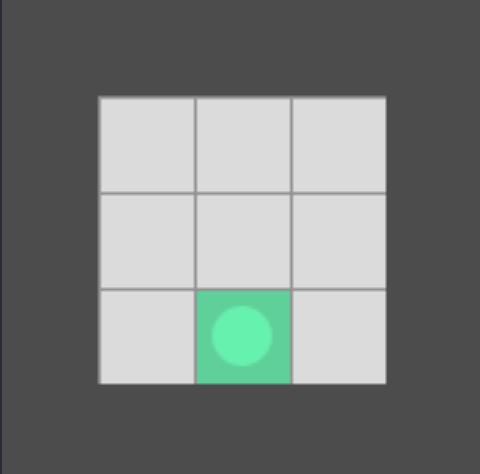
\includegraphics[width=1\linewidth]{1-agent-easy.png}\\
    \captionof{figure}[One Agent in a 5x5 Environment]{Visualization of a small environment with one agent}\label{fig:1-easy}
  \end{minipage}
  \hfill
  \begin{minipage}[b]{0.69\textwidth}
    \centering
    \begin{tabular}{lc}\hline
      Setting & Fully colored \\ \hline
        1 ppo & 3383 \\
        1 dqn & 650 \\ \hline
      \end{tabular}
      \captionof{table}[Training Results of one Agent in a 5x5 Environment]{Number of times the agent fully colored the environment during training with each learning algorithm. \\}\label{t:1-easy}
    \end{minipage}
  \end{minipage}\\\\

Table \ref{t:1-easy} shows the amount of times the grid on the left (Figure \ref{fig:1-easy}) was fully colored by one agent using each training algorithm. It is important to mention here, that the maximum step amount is set to 10 in both cases. The PPO agent colored the whole grid a total amount of 2130 times and the dqn agent 650 times.

\begin{figure}[hpbt]
    \centering
    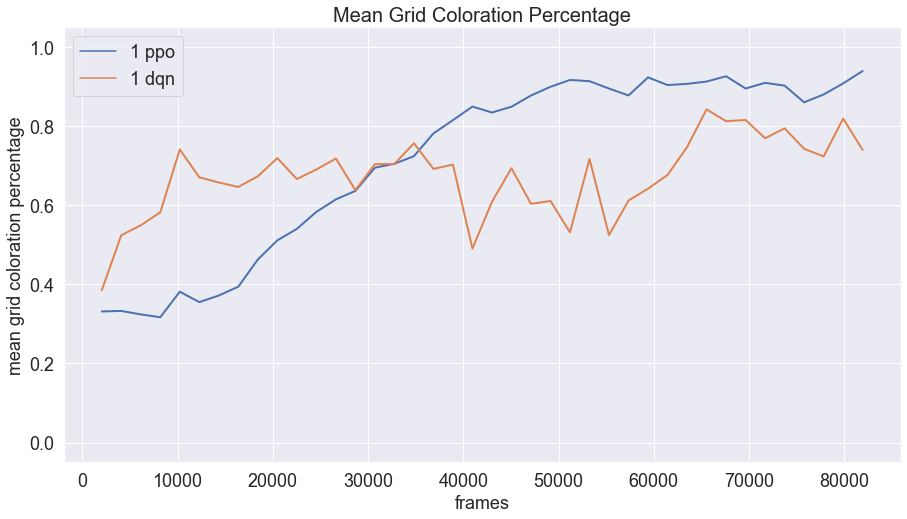
\includegraphics[width=0.8\textwidth]{1-easy-plot.png}\\
    \caption[Mean Coloration Percentage of one Agent in a small environment]{The mean coloration percentage of a 5x5 grid and one acting agent}\label{fig:1-easy-plot}
\end{figure}

The average grid coloration percentage of those settings is shown in plot \ref{fig:1-easy-plot}. The plot lines start at around 2048 frames, since this marks the first time a data entry of the parallel environments is returned. Furthermore, the plot exceeds the 80.000 default \verb|--frames|, since the last data entry includes the last data batch of the environments. The table shows, that both training runs solve the environment and the plot illustrates that in both cases generally a high percentage of the grid is colored. The dqn execution yields a better performance in the early stage, whereas the ppo agent gradually improves over time. In both cases an average coloration of over 70\% is eventually reached. This concludes that the grid is solvable with the parameters set.

\section{Easy Environment} \label{easy_env}

Now the multiagent scenario is compared. Here a set of two agents are trained to color the field of the same default dimensions, see Figure \ref{fig:2-coop-easy}. However, every agent executes an action during a step and with 10 steps and two agents in theory 20 cells could be visited. Hence, the \verb|--max-steps| count is reduced to 8. This should leave enough space for agents to make mistakes and still have a chance to solve the grid.

In order to get an overview of the overall 70 training results, the remaining 68 multiagent executions are divided into three different \verb|--setting| values. The first data division only covers the cooperation compositions, including ``difference-reward''. Table \ref{t:2-coop-easy} illustrates the scoreboard of the top three executions in this specification for each learning algorithm. \\\\

% ------------ COOP RESULTS ----------------
\begin{minipage}{\textwidth}
  \begin{minipage}[b]{0.29\textwidth}
    \centering
    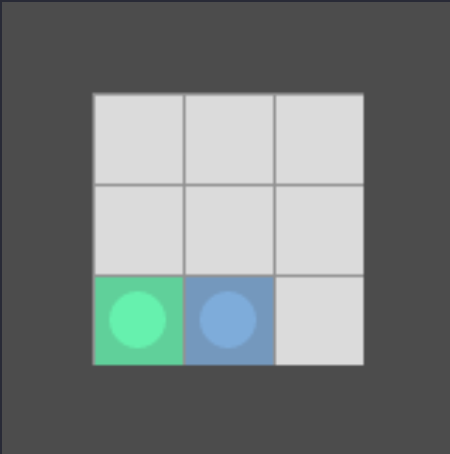
\includegraphics[width=1\linewidth]{2-agents-easy.png}\\
    \captionof{figure}[Two Agents in a 5x5 Environment]{Visualization of a small environment with two agents}\label{fig:2-coop-easy}
  \end{minipage}
  \hfill
    \begin{minipage}[b]{0.69\textwidth}
    \centering
    \begin{tabular}{clc}\hline
         & Top PPO Cooperation Settings & Fully colored \\ \hline
        {\small 1} & cooperation difference-reward & 1683 \\
        {\small 2} & cooperation & 1109 \\
        {\small 3} & cooperation sm-goal-no-reset & 533 \\ \hline
         &   \\ \hline
         & Top DQN Cooperation Settings & Fully colored \\ \hline
        {\small 1} & cooperation difference-reward & 5949 \\
        {\small 2} & cooperation am-goal-no-debt & 3197 \\
        {\small 3} & cooperation am-goal & 2880 \\ \hline
        \end{tabular}
        \captionof{table}[Training Results of two Cooperation Agents in a 5x5 Environment]{Number of times two agents working in cooperation fully colored the environment during training.}\label{t:2-coop-easy}
    \end{minipage}
  \end{minipage}\\\\

The measured attribute here is again the overall amount of fully colored states. In both cases the agents with the DR setting scored best, 1683 times with the PPO algorithm and 5949 times by using DQN. The PPO scores continue with the default cooperation scenario on second and the SM with the ``goal-no-reset'' condition on third place. 

On the contrary, the DQN results show AM settings on the remaining places, with the additions ``goal-no-debt'' on second place and ``goal'' on the third place. It is visible, that in both scoreboards the second and third executions are far behind the corresponding DR setting in terms of fully coloration counts.

\begin{figure}[hpbt]
    \centering
    %%----start of first subfigure----
    \subfloat[Reward summary of PPO agents]{
        \label{fig:2-ppo-coop-easy} %% label for first subfigure
        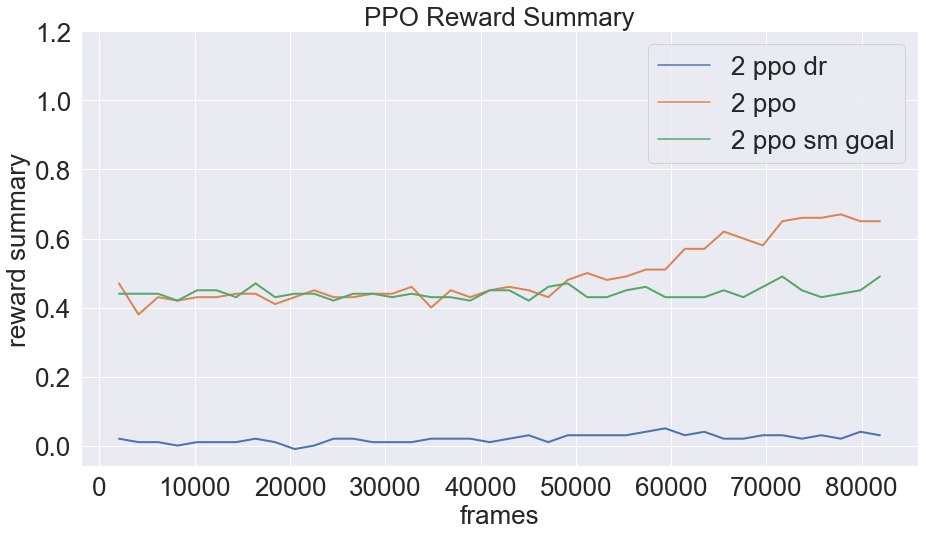
\includegraphics[width=0.48\linewidth]{2-ppo-easy.png}}
    \hspace{0.01\textwidth}
    %%----start of second subfigure----
    \subfloat[Reward summary of DQN agents]{
        \label{fig:2-dqn-coop-easy} %% label for second subfigure
        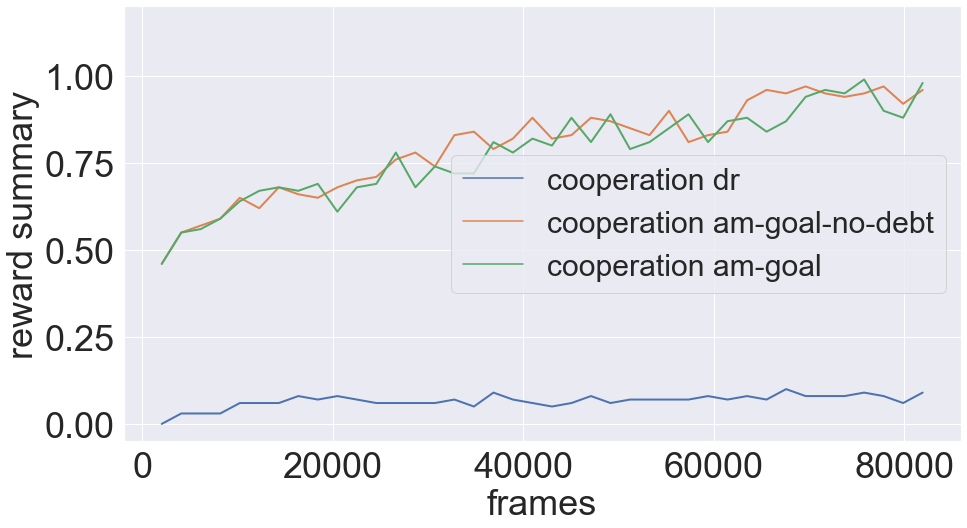
\includegraphics[width=0.48\linewidth]{2-dqn-easy.png}}
    \caption[Reward Summaries of the Top Cooperation Modes]{Reward Summaries of the top three cooperation compositions using PPO (left) and DQN (right)}
    \label{fig:multipic_plots_coop_easy} %% label for entire figure
\end{figure}

In the two plots of Figure \ref{fig:multipic_plots_coop_easy} the reward summary of the top scores, see table \ref{t:2-coop-easy}, are displayed. The term reward summary is used here, since the rewards of cooperating agents are equal and sometimes contain only slight changes through markets. However, in other agent compositions the rewards are rather specific to each agents' contribution. In any case the logged training data contains the mean reward of every agent separately. 

In order to summarize cooperation rewards, the average value of those separate agent rewards is calculated for each data entry and the results are then plotted here. For reward summaries of all other compositions each data entry is summarized with the sum of the separate agent rewards. The maximum y-axis label is set to 1.2, since agents get a reward of 1 if they color the whole field and additionally could get a reward of 0.1 for the final step. Through the reward summary calculations rounding errors may occur, which could in turn exceed the maximum reward of 1.1. Furthermore, markets could also contribute to bigger rewards. 

Even thought, the executions with the DR configuration scored highest in terms of reaching the goal, the reward lines in this case stay around 0.1. The reason for that is, that agents get the difference of two rewards, leading to very small values. All rewards, except the DRs, show a continuous increase and at least reach a summary reward of 0.8. 

The next training executions to look at are ``mixed-motive'' settings. Here again a scoreboard, listing the top three results of each learning algorithm, is shown in table \ref{t:2-mixed-easy}.
% ------------ MIXED RESULTS ----------------
\begin{center}
    \begin{tabular}{clc}\hline
         & Top PPO Mixed-Motive Settings & Fully colored \\ \hline
        {\small 1} & mixed-motive & 1734 \\
        {\small 2} & mixed-motive sm-no-reset & 1422 \\
        {\small 3} & mixed-motive sm-goal-no-reset & 1377 \\ \hline
         &   \\ \hline
         & Top DQN Mixed-Motive Settings & Fully colored \\ \hline
        {\small 1} & mixed-motive sm & 5417 \\
        {\small 2} & mixed-motive am-no-reset & 5379 \\
        {\small 3} & mixed-motive sm-goal & 5302 \\ \hline
        \end{tabular}
        \captionof{table}[Training Results of two Mixed-Motive Agents in a 5x5 Environment]{Number of times two agents working in a mixed-motive setting fully colored the environment during training.}\label{t:2-mixed-easy}
    \end{center}

The PPO scoreboard shows, that the plain ``mixed-motive'' setting is on the top with a score of 1734. Subsequently, SM configurations follow, with the addition of ``no-reset'' on second and ``goal-no-reset'' on third place. The DQN scores also show two SM settings, the default market occupies the first place here and the SM with the ``goal'' addition is on the last place, both however colored the grid a total of over 5300 times. The AM with the ``no-reset'' condition is on the second place in the DQN statistics.

\begin{figure}[hpbt]
    \centering
    %%----start of first subfigure----
    \subfloat[Mean trades of PPO agents]{
        \label{fig:2-ppo-mixed-easy} %% label for first subfigure
        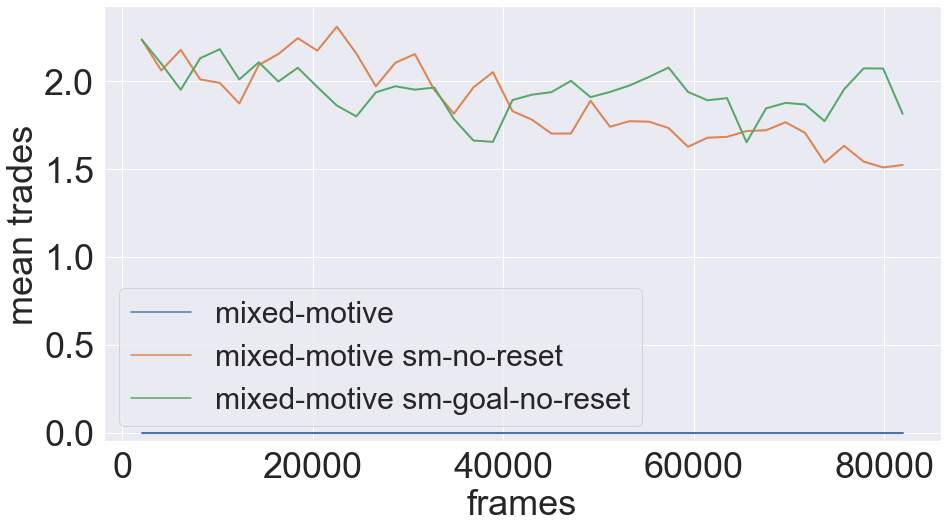
\includegraphics[width=0.48\linewidth]{2-ppo-mixed-easy.png}}
    \hspace{0.01\textwidth}
    %%----start of second subfigure----
    \subfloat[Mean trades of DQN agents]{
        \label{fig:2-dqn-mixed-easy} %% label for second subfigure
        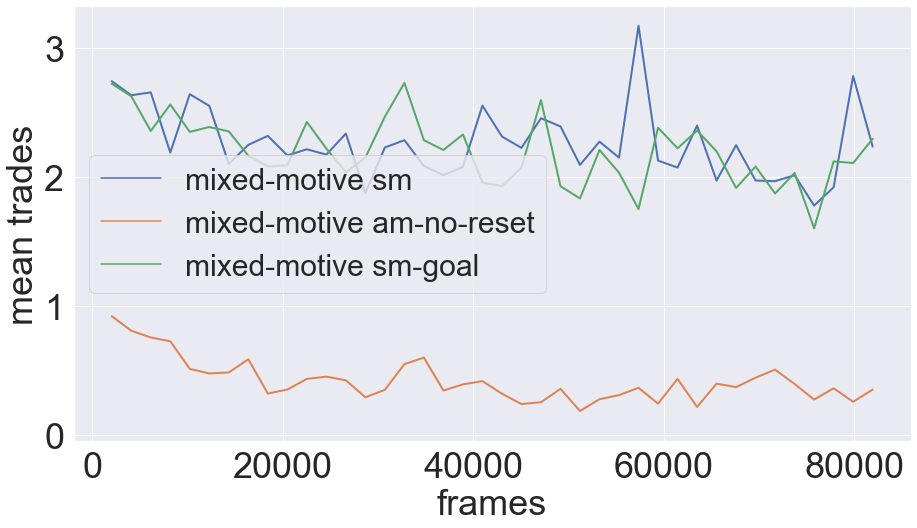
\includegraphics[width=0.48\linewidth]{2-dqn-mixed-easy.png}}
    \caption[Mean Trades of the Top Mixed-Motive Modes]{Mean trades of the top three mixed-motive compositions using PPO (left) and DQN (right)}
    \label{fig:multipic_plots_mixed_easy} %% label for entire figure
\end{figure}

In Figure \ref{fig:multipic_plots_mixed_easy} two plots are shown, visualizing the trading behavior of the agents during training. The plots display the mean amount of trades in the parallel environments. In plot \ref{fig:2-ppo-mixed-easy} the blue line stays at zero, since this execution does not contain a market extension. The other two lines are slightly decreasing and move between 2.2 and 1.5. Both lines here represent a SM interaction with the values showing that on average two market transactions occurred. This in turn means, that about two shares were bought in the completed episodes of all parallel environments.

In the right plot \ref{fig:2-dqn-mixed-easy} an AM is represented with the orange line. Here the mean trades are fewer compared to the other two SM lines. This is often the case for the two Markets, since action purchases subtract a bigger value at once, whereas selling shares reduces the payout over time. Comparing the SM executions between PPO and DQN shows, that the restriction of ``no-reset'' lowers the average trades to around 2, whereas without this specific condition the trade count is between 2 and 3.

The last dataset division only includes executions of competitive agent compositions. Table \ref{t:2-comp-easy} shows the scoreboards of this setup.

% ------------ COMP RESULTS ----------------
\begin{center}
    \begin{tabular}{clc}\hline
         & Top PPO Competitive Settings & Fully colored \\ \hline
        {\small 1} & competitive sm-goal-no-reset & 3614 \\
        {\small 2} & competitive & 3461 \\
        {\small 3} & competitive sm-goal & 3225 \\ \hline
         &   \\ \hline
         & Top DQN Competitive Settings & Fully colored \\ \hline
        {\small 1} & competitive sm-goal-no-reset & 7877 \\
        {\small 2} & competitive sm & 7842 \\
        {\small 3} & competitive am-goal-no-debt & 7560 \\ \hline
        \end{tabular}
        \captionof{table}[Training Results of two Competitive Agents in a 5x5 Environment]{Number of times two agents working in a competitive setting fully colored the environment during training.}\label{t:2-comp-easy}
    \end{center}

For both learning algorithms the most fully colored grids result from executions specifying a SM with the condition ``goal-no-reset''. In the DQN board follows the execution using the standard SM and the last place here is occupied by an AM with the specification ``goal-no-debt''. For PPO however the second place is the normal competitive mode without any additions and on third place is a SM execution with the ``goal'' restriction. Overall, the score differences within the tables are not big, at most a difference of around 300 goal states is observed. Furthermore, The scores of the first places in these two boards are the best values achieved so far, with 3614 fully colored grids in the PPO table and 7877 in the DQN table.

\begin{figure}[hpbt]
    \centering
    %%----start of first subfigure----
    \subfloat[Mean number of reset fields of PPO agents]{
        \label{fig:2-ppo-comp-easy} %% label for first subfigure
        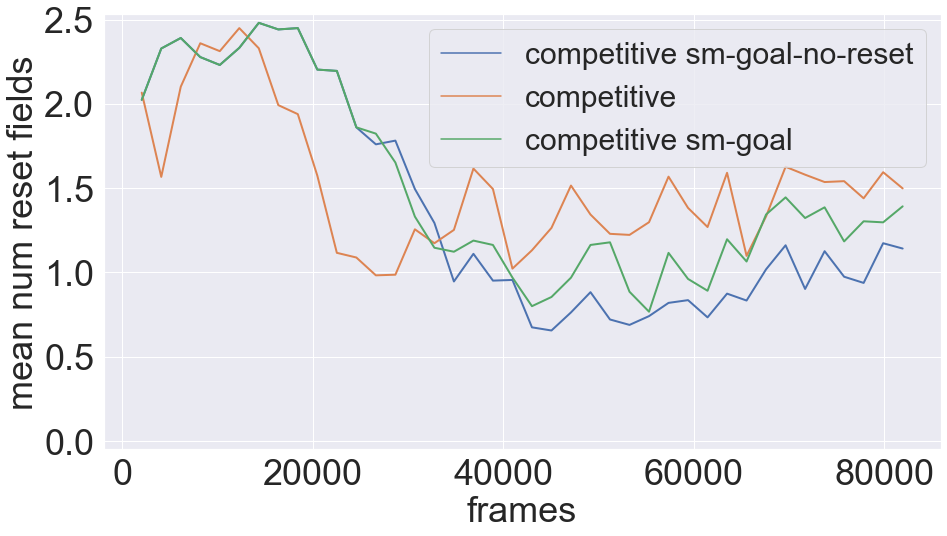
\includegraphics[width=0.48\linewidth]{2-ppo-comp-easy.png}}
    \hspace{0.01\textwidth}
    %%----start of second subfigure----
    \subfloat[Mean number of reset fields of DQN agents]{
        \label{fig:2-dqn-comp-easy} %% label for second subfigure
        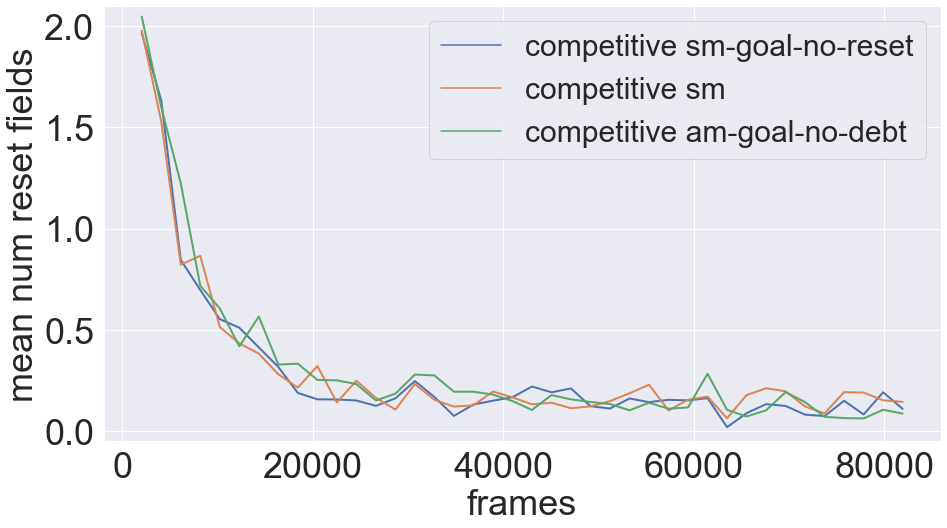
\includegraphics[width=0.48\linewidth]{2-dqn-comp-easy.png}}
    \caption[Mean Number of Reset Fields of the Top Competitive Modes]{Mean number of reset fields of the top three competitive compositions using PPO (left) and DQN (right)}
    \label{fig:multipic_plots_comp_easy} %% label for entire figure
\end{figure}

The plots to those scoreboards are displayed in Figure \ref{fig:multipic_plots_comp_easy}. In this case the average amount of reset fields are visualized. All lines start at a value two, which means, that during the first 2048 frames an average of two cells are reset during the completed episodes. In both cases the graphs eventually drop, however for PPO execution this takes around 20.000 frames and in the later half a small increase in all executions can be observed. Meanwhile, the three DQN trainings rapidly reduce the average resets to around 0.3. This value is never reached by PPO executions, here the lowest score is approximately 0.6.

\section{Difficult Environment} \label{difficult_env}
To see how the results change, when it becomes more challenging to reach the goal, all top executions showed before are now repeated in a bigger environment. The grid size is increased to 7 which provides an area of 5 by 5 for the agents to color. Also, since the grid offers more room the amount of agents is increased to 3.

To give the agents more time to learn the \verb|--frames| are set to 200.000 and the value of \verb|--frames-per-proc| is changed to 256. With the increase to 256 the training data entries are now 4096 frames apart instead of the 2048 we had before. The number 4096 comes from multiplying the number of environments with the \verb|--frames-per-proc|. To successfully solve the grid with one agent some DQN specific parameters needed to be tuned. As a result the adjusted values of \verb|--replay-size|, \verb|--epsilon-decay| and \verb|--target-update| are 700.000, 20.000 and 10.000. 

In Figure \ref{fig:1-hard} the one agent learning scenario in the difficult environment setup is shown. Here, the agent view size is also noticeable, with the lighter floor and wall colors three tiles around the agent. In this case the agent can not see the two top rows of the grid. This of course also contributes to the difficulty of this setup. \\

\begin{minipage}{\textwidth}
  \begin{minipage}[b]{0.29\textwidth}
    \centering
    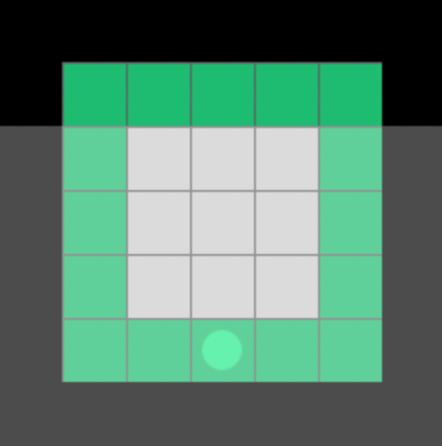
\includegraphics[width=1\linewidth]{1-agent-hard.png}\\
    \captionof{figure}[One Agent in a 7x7 Environment]{Visualization of a 7x7 Environment with one agent}\label{fig:1-hard}
  \end{minipage}
  \hfill
  \begin{minipage}[b]{0.69\textwidth}
    \centering
    \begin{tabular}{lc}\hline
      Setting & Fully colored \\ \hline
        1 ppo & 2924 \\
        1 dqn & 394 \\ \hline
      \end{tabular}
      \captionof{table}[Training Results of one Agent in a 7x7 Environment]{Number of times the agent fully colored the environment during training with each learning algorithm.\\ }\label{t:1-hard}
    \end{minipage}
  \end{minipage}\\\\

The results of the training executions with one agent are shown in table \ref{t:1-hard}. Similar to the easier setup, the PPO training results in more fully colored grids compared to the DQN execution. While the PPO agent reaches the goal 2924 times the DQN agent only achieves 394 goal states. Comparing those numbers with their corresponding easy equivalent it is obvious that for both learning algorithms the scores have decreased.

\begin{figure}[hpbt]
    \centering
    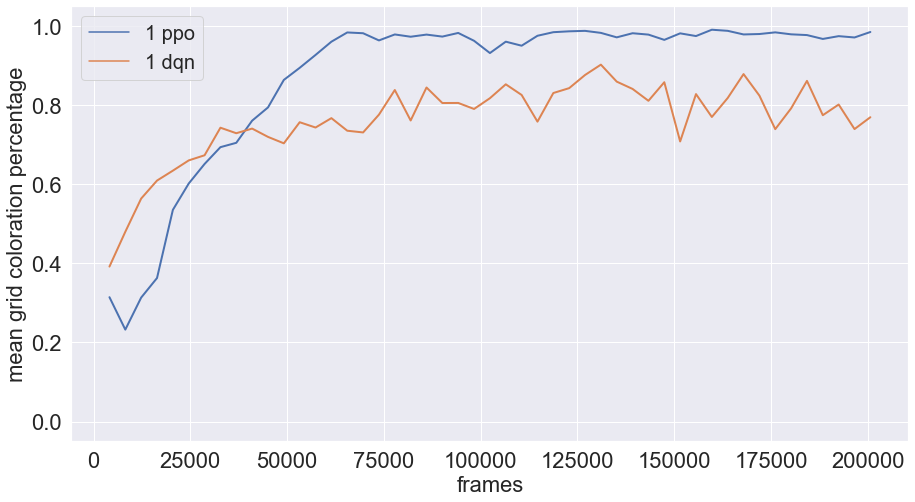
\includegraphics[width=0.8\textwidth]{1-hard-plot.png}\\
    \caption[Mean Coloration Percentage of one Agent in a 7x7 Environment]{The mean coloration percentage of a 7x7 grid and one acting agent}\label{fig:1-hard-plot}
\end{figure}

Looking at the mean coloration percentage plot \ref{fig:1-hard-plot} however, both executions show an increase to a relatively high percentage. The DQN agent training reaches an average of 80\% grid coloration and deviates only slightly around it. In comparison, the training with PPO has a steep incline from 20 to 95\% and after 60.000 frames this high amount is maintained until the end of training. This proves again that both algorithms can solve the environment with the set parameters.


\begin{minipage}{\textwidth}
  \begin{minipage}[b]{0.29\textwidth}
    \centering
    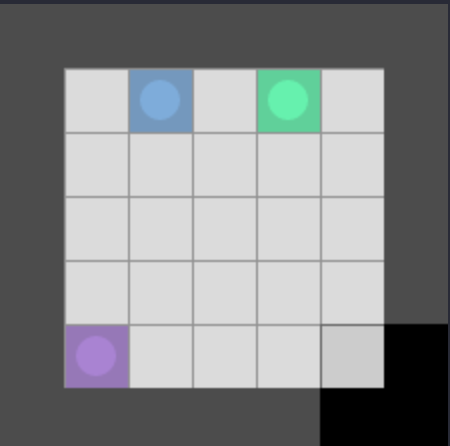
\includegraphics[width=1\linewidth]{3-agents-hard.png}\\
    \captionof{figure}[Three Agents in a 7x7 Environment]{Visualization of a 7x7 environment with three agents}\label{fig:3-hard}
  \end{minipage}
  \hfill
    \begin{minipage}[b]{0.69\textwidth}
    \centering
    \begin{tabular}{clc}\hline
         & Top PPO Cooperation Settings & Fully colored \\ \hline
        {\small1} & cooperation difference-reward & 166 \\
        {\small2} & cooperation & 10 \\
        {\small3} & cooperation sm-goal-no-reset & 0 \\ \hline
         &   \\ \hline
         & Top DQN Cooperation Settings & Fully colored \\ \hline
        {\small 1} & cooperation difference-reward & 115 \\
        {\small 2} & cooperation am-goal-no-debt & 0 \\
        {\small 3} & cooperation am-goal & 0 \\ \hline
        \end{tabular}
        \captionof{table}[Training Results of three Cooperation Agents in a 7x7 Environment]{Number of times three agents working in cooperation fully colored the environment during training. \\}\label{t:2-coop-easy}
    \end{minipage}
  \end{minipage}\\\\

  \begin{center}
    \begin{tabular}{clc}\hline
         & Top PPO Mixed-Motive Settings & Fully colored \\ \hline
        {\small 1} & mixed-motive & 247 \\
        {\small 2} & mixed-motive sm-goal-no-reset & 133 \\
        {\small 3} & mixed-motive sm-no-reset & 66 \\ \hline
         &   \\ \hline
         & Top DQN Mixed-Motive Settings & Fully colored \\ \hline
        {\small 1} & mixed-motive sm-goal & 116 \\
        {\small 2} & mixed-motive sm & 42 \\
        {\small 3} & mixed-motive am-no-reset & 31 \\ \hline
        \end{tabular}
        \captionof{table}[Training Results of three Mixed-Motive Agents in a 7x7 Environment]{Number of times three agents working in a mixed-motive setting fully colored the environment during training.}\label{t:2-comp-easy}
    \end{center}

    \begin{center}
    \begin{tabular}{clc}\hline
         & Top PPO Competitive Settings & Fully colored \\ \hline
        {\small 1} & competitive & 277 \\
        {\small 2} & competitive sm-goal & 165 \\
        {\small 3} & competitive sm-goal-no-reset & 111 \\ \hline
         &   \\ \hline
         & Top DQN Competitive Settings & Fully colored \\ \hline
        {\small 1} & competitive sm-goal-no-reset & 367 \\
        {\small 2} & competitive sm & 240 \\
        {\small 3} & competitive am-goal-no-debt & 198 \\ \hline
        \end{tabular}
        \captionof{table}[Training Results of three Competitive Agents in a 7x7 Environment]{Number of times three agents working in a competitive setting fully colored the environment during training.}\label{t:2-comp-easy}
    \end{center}